\documentclass[a5paper]{report}

\usepackage{amsmath, amssymb}
\usepackage[margin=0.75in]{geometry}
\usepackage{graphicx}
\graphicspath{ {../../Images/ENEG11009/} }
\usepackage[breaklinks]{hyperref}
\usepackage{tikz}
\usepackage{stix}

\begin{document}
	\begin{titlepage}
		\centering
		{\Huge \textsc{ENEG11009}\par}
		\vspace{1cm}
		{\Large \textsc{The Weekly Notes}\par}
		\vspace{2.5cm}
		\vfill
		Authored by\par
		Lachlan J. W. Wyer
		\vfill
		{\large Document Date: \par}
		\date{16/09/2025}
		{\large \today\par}
	\end{titlepage}
	\section*{Week 1 - Energy \& Energy Conservation}
	\subsection*{Energy:}
	Energy is the ability to work, either physical or mental. It does not matter if this work is self-contained or used up in a system. In a closed system, there is a fixed about of total energy within the closed system, that does not interact with anything outside of the system. The main SI unit for energy is Joules (J).
	\subsection*{Types of Energy:}
	\subsubsection*{Kinetic Energy ($E_{KE}\;\text{or}\;K_{E}$):}
	This energy is the energy of motion. Implying that all moving objects contain a form of $K_{E}$, e.g. The wind or water.\\
	As shown in $K_{E}$'s equation, the heavier or faster an object is, the greater the its $K_{E}$. As such, kinetic energy comes in two main forms:
	\begin{itemize}
		\item Translational $K_{E}$: The motion along a specified path
		\item Rotational $K_{E}$: The motion around an axis
	\end{itemize}
	As such the formula for kinetic energy can be derived from both the object mass and velocity.
	$$K_{E}\;\alpha\;m\;\;\&\;\;K_{E}\;\alpha\;v^{2}$$
	$$\therefore\;K_{E}=\frac{1}{2}mv^{2}$$
	\begin{itemize}
		\item $K_{E}$ - Joules
		\item m - Mass of the object(kg)
		\item v - velocity of the object ($\frac{m}{s}$)
	\end{itemize}
	\subsubsection*{Potential Energy ($E_{PE}$):}
	This is a type of stored energy that can readily be converted into another form. For example the water store behind a dam, or thermal vents. There are three main types of potential energy: gravitional, elastic and thermal.
	\subsubsection*{Gravitional Potential Energy ($G_{PE}$):}
	This type of energy is the type of stored energy associated with objects height \& mass.
	$$E_{PE}=mgh$$
	\begin{itemize}
		\item $G_{PE}$ - Joules (J)
		\item $m$ - mass of the object, can also be calculated from an object's forces ($F=mg$)
		\item $g$ - Standarized gravity ($9.8m\;s^{-1}$)
		\item $h$ - Height (m)
	\end{itemize}'
	\subsection*{Elastic Potential Energy ($E_{PE}$):}
	$$E_{PE}=\frac{1}{2}kx^{2}$$
	\begin{itemize}
		\item $E_{PE}$ - Joules of energy
		\item $k$ - The spring of elastic constant ($\frac{N}{m}$)
		\begin{itemize}
			\item This constant can also be calculated($k=-\frac{F_{s}}{x}$)
		\end{itemize}
		\item $x$ - The displacement of the object(m)
	\end{itemize}
	\subsection*{Thermal Energy ($E_{TH}$):}
	This energy is created due to movement of particles. The hotter a substance, the more its particles move. Also, the greater its friction co-efficient the more the substance will heat up, and thus the $E_{TH}$ will increase.
	$$E_{TH}=f_{F}x$$
	\begin{itemize}
		\item $E_{TH}$ - Measured in Joules (J)
		\item $f_{F}$ - The friction created in movement ($f_{F}=\mu mg$)
		\item $x$ - The distance moved an object
	\end{itemize}
	\begin{center}
		OR
	\end{center}
	$$E_{TH}=\mu mgx$$
	\begin{itemize}
		\item $\mu$ - The friction coefficient of the floor
		\item $m$ - The mass of object (kg)
		\item $g$ - Gravitional Constant ($9.8m\;s^{-1}$)
	\end{itemize}
	\subsection*{Force:}
	Force can be split into two main types:
	\begin{enumerate}
		\item Conservative
		\begin{itemize}
			\item Independent of a Path
			\item Contains and stores useful energy
		\end{itemize}
		\item Non-conservative
		\begin{itemize}
			\item Dependent on a specific path
			\item Cannot store useful energy
		\end{itemize}
	\end{enumerate}
	\subsection*{Energy Transformations:}
	According to Newton's First Law, energy can neither can be created nor destroyed, only transformed from one form to another. As such, the total energy remains the same within a closed system. In the end it will only be converted into undesirable forms. Energy can be transferred between a system and its environment, through two main ways.
	$$E_{Total}=K_{E}+E_{PE}+G_{PE}+E_{TH}+\ldots +W$$
	\begin{enumerate}
		\item Work: Mechanical transfer of Energy, e.g. Pushing or Pulling
		\item Heat: Non-mechanical transfer of Energy, e.g. A temperature difference between objects
	\end{enumerate}
	\subsection*{Work:}
	Work is done when a force is applied over a distance.
	$$W = \vec{F}\cdot \vec{d}$$
	\begin{itemize}
		\item W \- Work is a scalar product (J or $N\cdot m$)
		\item The vectors $\vec{F}\text{(N)}$ and $\vec{d}\text{(m)}$ must ve in the same direction or have them resolved into a parrallel directions.
	\end{itemize}
	E.g. A crate is 500cm with a force of 500N
	\begin{eqnarray*}
		W &=& \vec{F}\cdot \vec{d} \\
		  &=& 500\cdot 500\times10^{-2} \\
		  &=& 2500J \\
		  &=& 2.5kJ
	\end{eqnarray*}
	\subsection*{Power:}
	Power can be described as an amount of energy convertted (the work done) per unit of time. The unit of time is usually seconds.
	$$P=\frac{W}{t}\;\;\text{OR}\;\;P=\frac{E}{t}$$
	The SI unit of P is $\frac{J}{s}$ or W(Watts).\\
	A different way of calculating an instaneous output:
	$$P=\frac{W}{t}=\frac{\vec{F}\cdot\vec{d}}{t}=\vec{F}\cdot\frac{\vec{d}}{t}=\vec{F}\cdot v$$
	\subsection*{Efficiency:}
	Inessence, basically nothing can possibly be 100\% efficient. Reductions can be found in:
	\begin{itemize}
		\item Process limitations: Practical implementation within the realworld
		\item Fundamental limitations: The laws of physics and the realworld
	\end{itemize}
	A system can have lower efficienies can be due to increase in energy losses.
	$$\eta = \frac{Useful Energy Transferred}{Total Energy Supplied} \times 100$$
	\begin{itemize}
		\item $\eta$ - The efficiency of a system (\%)
	\end{itemize}

	\section*{Week 2 - Heat \& Gas}
	\subsection*{$0^{\text{th}}$ Law of Thermodynamics:}
	This law states that two systems can be considered in thermal equilibrium, iff there is on net flow of $E_{TH}$ between the systems when a path is connected that allows flow. When two systems in thermal equilibrium can be assumed to have the same temperature.\\
	$E_{TH}$: The internal energy of a system due to temperature.\\
	Temperature: Average $K_{E}$ of the atoms that make up an ideal gas.

	\subsection*{Temperature Scales:}
	$$^{o}C->^{o}F:\frac{9}{5}^{o}C+32$$
	$$^{o}C->K:\;^{o}C+273$$
	The Kelvin and Celsius scales are considered to be almost thermally equal. Meaing that when one is change by an amount (e.g. 1K) the other change by the same (e.g. $1^{o}$C).

	\subsection*{Heat (Q):}
	Heat is considered to be the energy transferred across the boundary of 2 different systems because of a temperature difference. Heat has different methods of exchanging energy with objects \& their surrounds:
	\begin{itemize}
		\item Conduction: Mostly in solids without the movements of mass
		\item Convection: Generally in liquids or gases, and the transfer involves movement of mas
		\item Radiation: Does not need a medium to transfer heat, e.g. heat can be transferred in a vaccum
		\item Evaporation; Molecules movings through states, e.g. Liquid -> Gas below the molecules boiling point
	\end{itemize}

	\subsubsection*{Conduction}
	The transfer of thermal energy between connected materials.
	$$Q\;\alpha\;\Delta T, \text{where}\;\Delta T=T_{H}-T_{C}$$
	$$Q\;\alpha\;A, \text{where}\;A=CSA$$
	$$Q\;\alpha\;\frac{1}{L}, \text{where L is the length between molecules}$$
	As such the equation for conduction is as follows:
	$$P_{cond}=\frac{Q}{t}=\frac{kA \Delta T}{L}$$
	\begin{itemize}
		\item $P_{cond}$ - In Watts
		\item $k$ - The thermal conductivity of the object ($\frac{W}{m}\cdot K$)
		\item $A$ -  Is the the CSA
		\item $\Delta T$ - The temperature difference
		\item $L$ - THe Thickness between the molecules or length of the object
	\end{itemize}

	\subsubsection*{Radiation}
	$$P_{rad}=\frac{Q}{\Delta T}=e\sigma A(T_{1}^{4}-T_{2}^{4})$$
	\begin{itemize}
		\item $e$ - The emmisivity of a particular surface (0->1)
		\item $\sigma$ - The Stefen-Boltzmann constant ($5.67\times 10^{-3} \frac{W}{m^{2}}\cdot K^{4}$)
		\item $A$ - CSA
		\item $T_{1}^{4}\;\text{or}\;T_{2}^{4}$ - The temperature measured in Kelvin
	\end{itemize}

	\subsection*{Specific Heat Capacity:}
	The quantity of heat absorbed to increase 1kg of substance increase 1K.
	$$Q=mc\Delta T$$

	\subsection*{Atomic Model of Matter:}
	Solid:
	\begin{itemize}
		\item Particles are connected with strong, spring-like bonds
		\item The particles have a defined shape
		\item Can be compressed slightly
	\end{itemize}
	Liquid:
	\begin{itemize}
		\item Weak bonds present between particles
		\item Particles can move slightly
		\item Takes the shape of the container that it is placed in, e.g. bowl.
	\end{itemize}
	Gas:
	\begin{itemize}
		\item No inter-molecular bonds are present
		\item Particles are in random motion
		\item Particles interact with elastic collisions
		\item Move freely \& fill the entire vessel they are placed in
	\end{itemize}
	When molecules change phase, heat is still being transferred with no temperature change. The amount of heat required for this called latent heat.

	\subsection*{Latent Heat:}
	There are two types of latent heat, 1. Heat of Fusion and 2. Heat of vaporization. Heat of fusion ($L_{F}$) is the amount of heat required to convert all 1kg of substance from a solid to a liquid. Heat of vaporization ($L_{v}$) is similar except it requires changing from a liquid to a gas. The SI unit for this is $\frac{kJ}{kg}$.
	$$Q=mL$$
	\begin{itemize}
		\item $Q$ - Heat required to change phase. This can either be $\pm$
		\item $m$ - The mass of the substance changing states
		\item $L$ - The Latent required to change state
	\end{itemize}

	\subsection*{$1^{st}$ Law of Thermodynamics:}
	The change in energy is the difference between the heat added \& the work done.
	$$\Delta U=U_{f}-U_{i}=Q-W$$
	If $Q\;>\;0$, heat has been added to system. Else $W\;>\;0$, work has been done by the system.

	\subsection*{$2^{nd}$ Law of Thermodynamics:}
	Entropy (s) always increases, as it is an irreversible process. Everything in order will always lead to disorder.
	$$\Delta s=\frac{\Delta Q}{T}$$

	\subsection*{Energy Reservior:}
	A system with a huge heat capacity (whether hot or cold) that does not change in temperature when a change in heat happens. For example, adding 1L of boiling water to the ocean does not "really" change the temperature of the ocean. Even though alot of heat has been added into the ocean.

	\subsection*{Pressure:}
	The value of pressure is a force applied $\perp$ to the surface area of a contianer or vessel. The SI unit is $1Pa=1\frac{N}{m^{2}}=1\frac{kg}{m\;s^{-2}}$. Other unit conversions to remember are $1atm=101,300Pa=14.7psi$.
	$$p\;\alpha\;T,\;\;\;p\;\alpha\;\frac{1}{V},\;\;\;p\;\alpha\;n$$
	$$pV=nRT$$
	\begin{itemize}
		\item $p$ - Pa
		\item $V$ - $m^{3}$
		\item $n$ - moles of substance
		\item $R$ - The real gas constant ($8.31\;\frac{J}{mol}\cdot K$)
		\item $T$ - Temperature in Kelvin
	\end{itemize}
	
	\section*{Week 3 - Electricity}
	\subsection*{SI Units used:}
	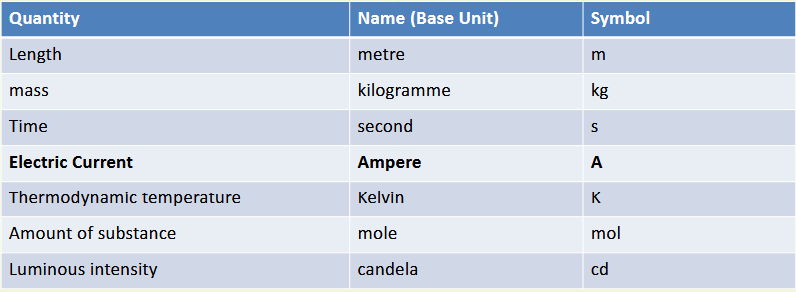
\includegraphics[width=4in]{SI-Units.png}

	\subsection*{Amps:}
	The charge of an electron is $1.602\;176\;634\times 10^{-19}$C. The amps in a circuit can be defined as the quantity of charge passing through a cross-section per unit time.
	$$I=\frac{Q}{t}$$
	\begin{itemize}
		\item $Q$ - The unit for measuring charge is Coulomb (C)
		\item $t$ - Time (seconds)
	\end{itemize}

	\subsection*{Voltage:}
	The voltage of a system is the difference in potential between elements in the circuit. Voltage is related to Amps through it having $\frac{\text{Joules}}{\text{Coulomb}}$.
	$$V=\frac{W}{I}=\frac{J/t}{I}=\frac{J}{It}$$

	\subsection*{Conductors:}
	Conductors are a material that allows free movement of charge. For example allows current to flow through it, like every metal is basically a conductor. Conductors work through having the conduction and valence electron bands overlapping. This means that little to no energy is required to change bands.
	\begin{center}
		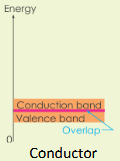
\includegraphics[scale=2]{conductors.png}
	\end{center}

	\subsection*{Insulator:}
	Insulators are materials that prevent the free movement of charge. Examples of insulators are rubber, ceramic, cork, and air. They work through the conduction and valence bands having an energy gap. This is because to change energy levels require large amount energy.

	\subsection*{Semi-conductors:}
	Semi-conductors are a crystalline material that has properties between a conductor and insulator.

	\subsection*{Resistance:}
	The resistivity of a material is mesaured in how strongly it resists an electrical current.
	$$\sigma = \frac{1}{\rho}$$
	The resistance of a material is a property of a specific wire that depends on of factors.
	$$R\;\alpha\;L,\;\;\;R\;\alpha\;\frac{1}{A}$$
	$$R=\frac{\rho L}{A},\;\;\;\;\rho =\frac{RA}{L}$$
	\begin{itemize}
		\item R - Ohms ($\Omega$)
		\item $\rho$ - Restivity ($\Omega\cdot m$)
		\item L - Length of material ($m$)
		\item A - CSA of material ($m^{2}$)
	\end{itemize}
	\begin{center}
		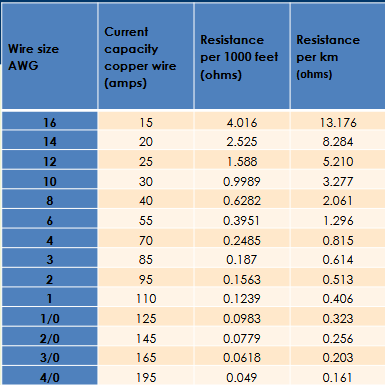
\includegraphics{wire-gauge.png}
	\end{center}

	\subsection*{Electrical Circuit Elements:}
	The voltage values within a circuit should follow the positive sign convention. $+\rightarrow -$ voltage, there is considered to be a voltage drop between the two points. For current, the current coming into the node has to equal the current leaving.

	\subsection*{Ohm's Law:}
	According to this law, the current flowing through a material is proportional to its voltage, e.g. $I\;\alpha\;V$.
	$$\therefore\;I=\frac{V}{R}\;\;OR\;\;V=IR\;\;OR\;\;R=\frac{V}{I}$$

	\subsection*{Equivalent Resistance:}
	Things to remember:\\
	If a circuit is connected in series, all elements have the same current and share the voltage.
	$$R_{eq}=\sum_{i=1}^{n}R_{i}$$
	\begin{center}
		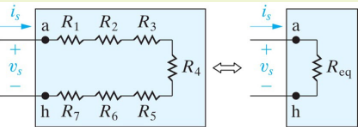
\includegraphics{req-series.png}
	\end{center}
	Whereas, connected in parrellel, they contain the same voltage and share current.
	$$Req=\frac{1}{\sum_{i=1}^{n}\frac{1}{R_{i}}}=(\sum_{i=1}^{n}\frac{1}{R_{i}})^{-1}$$
	\begin{center}
		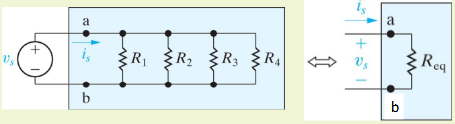
\includegraphics{req-parrallel.png}
	\end{center}

	\subsection*{Kirchoff's Laws:}
	\subsubsection*{Current (KCL)}
	The sum of all within a node must equal 0. Therefore, the current entering a node must be equal to that exiting.
	\begin{eqnarray*}
		-I_{In}+I_{Out} &=& 0 \\
		\sum I_{In} &=& \sum I_{Out}
	\end{eqnarray*}

	\subsubsection{Voltage (KVL)}
	The sum of all voltage differences within a circuit (or a specific closed loop) must be 0.
	$$\sum_{i=0}^{n}V_{i}=0$$

	\section*{Week 4 - Rotational Motion \& AC Power}
	\subsection*{Rotational Motion:}
	$$\theta (\text{rad})=\frac{s}{r}$$
	This is the defition of a radian. Remember Specialist and Methods converstions between radians and degrees. It is important to remember that rotational motion happens about the turn of a central/interal axis. Rotional motions comes in two forms:
	\begin{enumerate}
		\item Linear Motion\\
		$x=v_{0}t+\frac{1}{2}at^{2}$, where:
		\begin{itemize}
			\item $x$ - The displacement along an axis
			\item $v_{0}$ - An object's initial velocity
			\item $a$ - The acceleration of an object
			\item $t$ - Time (secs)
		\end{itemize}
		\item Angular Velocity\\
		$\omega = \frac{\Delta\theta}{\Delta t}$, where:
		\begin{itemize}
			\item $\omega$ - $\frac{rad}{s}$
			\item $\Delta\theta$ - Change in radians
			\item $\Delta t$ - Amount of times to take the change
		\end{itemize}
	\end{enumerate}

	The angular velocity is just the derivative with respect to time of the angular position. Other units can also be used, e.g. RPM, but must be converted to $\frac{rad}{s}$ for these equations. For rotation motion, the time to complete one rotation is the period of motion (T). Compared to the number of revolution per seconds is the frequency (f).
	$$f=\frac{1}{T}$$
	$$\omega=2\pi f$$
	
	\subsection*{Angular Speed:}
	$$v=r\omega$$
	
	\subsection*{Angular Displacement:}
	\subsubsection*{Linear Displacement}
	$$x_{f}-x_{i}=\Delta x=v_{x}\Delta t$$
	\subsubsection*{Angular Displacement}
	$$\Delta\theta=\theta_{f}-\theta_{i}=\omega\Delta t$$

	\subsection*{Rotation of a Rigid Body:}
	A rigid body is an object that does not change shage when motion is being taken. For example, types of rigid body motion is shown in the image below.
	\center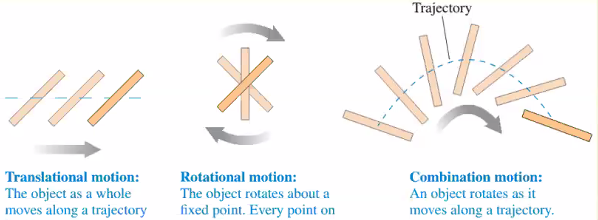
\includegraphics{type-RBM.png}\\
	\raggedright{Just some equations to understand}\\
	\center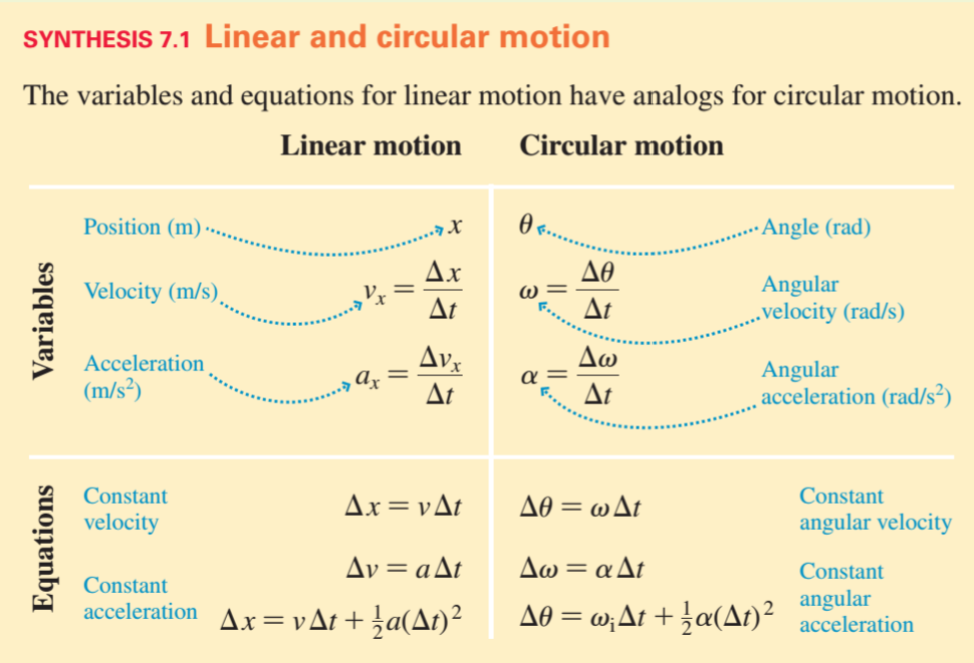
\includegraphics[scale=0.5]{equations-1.png}\\
	\raggedright

	\subsection*{Tangential (Linear) Acceleration:}
	$$a_{t}=\frac{\Delta v}{\Delta t}=\frac{\Delta(\omega r)}{\Delta t}=\alpha r$$
	Centripital acceleration is $\perp$ to its $\vec{v}$ \& aims towards the centre.

	\subsection*{Torque:}
	Torque is the measure of the effectiveness of a force at causing an object to rotate around a pivot.
	$$\tau = r\cdot Fsin(\phi)=-r_{\perp}mg$$
	\begin{itemize}
		\item $\tau$ - Torque ($N\cdot m$)
		\item r - Distance (m)
		\item F - Force (N)
		\item $\phi$ - Angle of movement, required as the force must be $\perp$ to the object or resolved
	\end{itemize}
	The $\tau_{net}=\sum T=\alpha I$, where $I$ is the moment of ineritia.
	$$I(kg\cdot m^{2})=\sum m_{i}r_{i}^{2}$$
	And Newton's $2^{nd}$ Law of rotational motion states that $\alpha = \frac{\tau_{net}}{I}$.\\
	As such, some more rotational dynamics items to know are:\\
	\center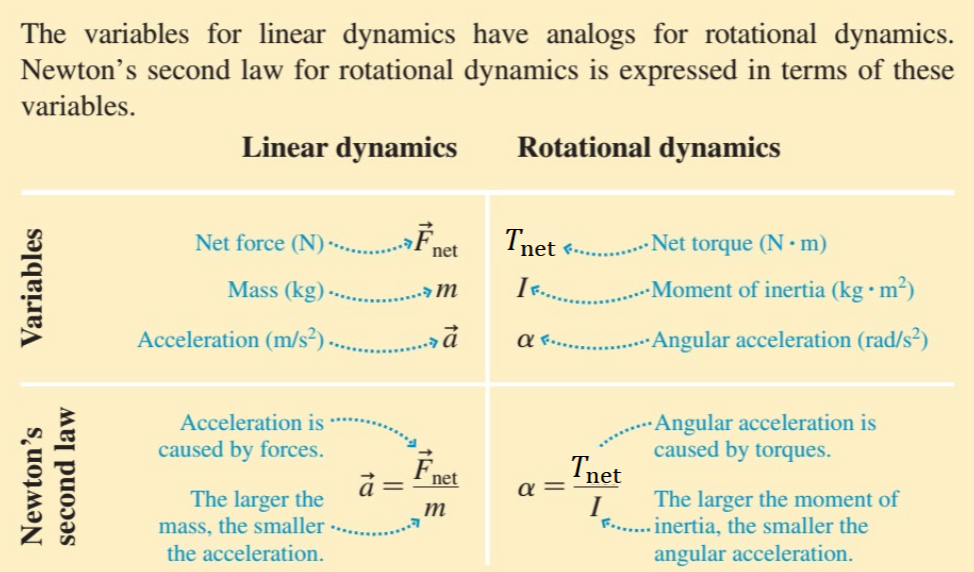
\includegraphics[scale=0.70]{rotational-dynamics.png}

	\raggedright\subsection*{AC Power:}
	Power can be converted between AC and DC power profiles. DC is a constant voltage overtime, e.g. 12V DC is always 12V. Whereas, 12V rotates between +12V \& -12V, because AC alternates polarity overtime.\\
	The default AC waveform is the sinusoidal waveform.\\
	\begin{center}
		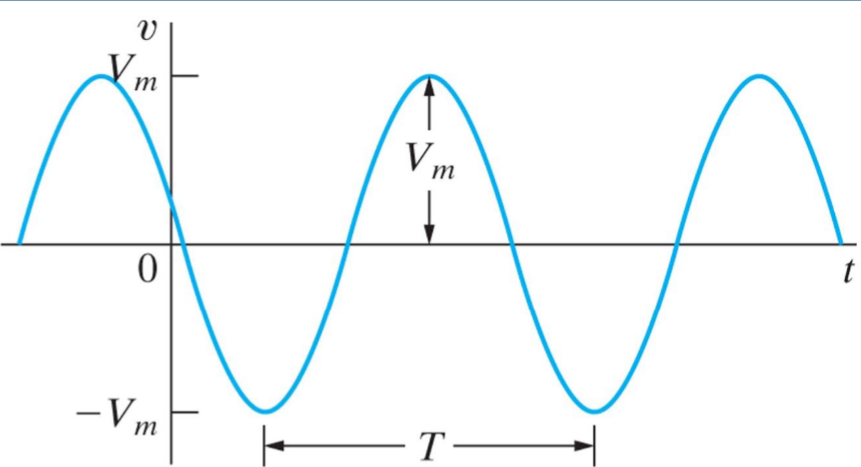
\includegraphics[scale=0.75]{sinusodial-waveform.png}
	\end{center}
	$$v(t)=V_{m}sin(\omega t + \psi)=V_{m}cos(\omega t +\phi)$$
	The phase angle ($\psi,\;\phi$) defines the value of v(t) @ t=0. Positive values shift the graphs left, whilst negative values shift right.
	
	\subsection*{Resistors:}
	In a resistor circuit: $v_{source}(t)=v_{R}(t)$.\\
	Here max amps and max voltage happens at the same time. With this it could be said that current is in phase with the voltage.
	\begin{center}
		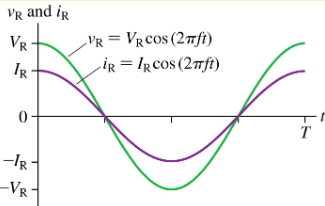
\includegraphics[scale=1.5]{resistor-graph.png}
	\end{center}

	\subsection*{Capacitor:}
	$$v_{C}(t)=V_{C}sin(2\pi ft),\;\;\text{Assuming that}\;\phi\;=\;0$$
	In the capacitor graph, the current in leading the voltage by $\frac{\pi}{2}$.
	\begin{center}
		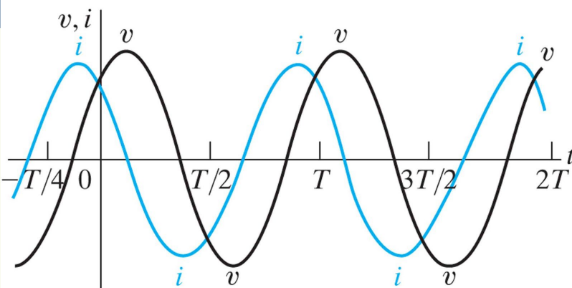
\includegraphics{capacitor-graph.png}
	\end{center}
	$$X_{C}=\frac{1}{\omega_{C}}=\frac{1}{2\pi ftc}$$

	\subsection*{Inductor:}
	For this, assume that the inductor is connected too the wave source.
	$$i_{L}=I_{L}cos(2\pi ft)$$
	Here the current is lagging the voltage by $\frac{\pi}{2}$
	\begin{center}
		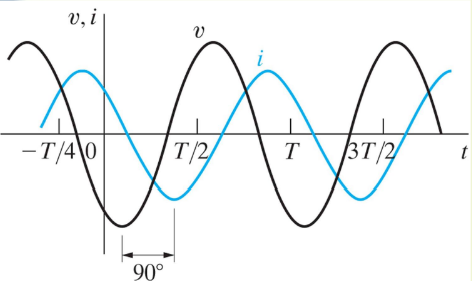
\includegraphics{inductor-graph.png}
	\end{center}
	$$X_{L}=\omega L=2\pi fL$$

	\subsection*{Relationships:}
	To remember the units and styles see the image below.
	\begin{center}
		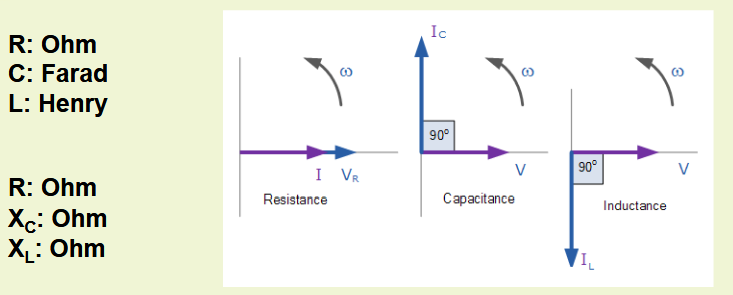
\includegraphics[scale=0.8]{relationships-graph.png}
	\end{center}

	\subsection*{Root Mean Square (RMS):}
	The RMS value is useful because AC can then be compared DC directly. Thus, AC RMS values can be compared against DC values, creating a heating a value (e.g. power and heat).\\
	\subsubsection*{Resistor:}
	$$V_{RMS}=I_{RMS}R$$
	$$v_{RMS}(t)=I_{RMS}(t)\cdot R$$
	\subsubsection*{Capacitor:}
	$$V_{RMS}=I_{RMS}\times\frac{1}{Q_{C}}$$
	$$v_{C}(t)=I_{C}(t)\cdot X_{C}$$
	\subsubsection*{Inductor:}
	$$V_{RMS}=I_{RMS}\omega L$$
	$$v_{L}(t)=I_{L}(t)\cdot X_{L}$$

	\section*{Week 5 - Generators:}
	\subsection*{DC Generators}
	All DC generators have a voltage induced across a conductor, where an inductor through a magnetic field. This phenomeoa is calld electromagnetic induction. To cause this relative motion is all that is needed. Whether the conductor or the magnet can move. The official name for this is called Faraday's Law.\\
	There are several ways in which DC generators can be classified. For example, the simpliest DC generator, powered through a permenant magnet.
	\begin{center}
		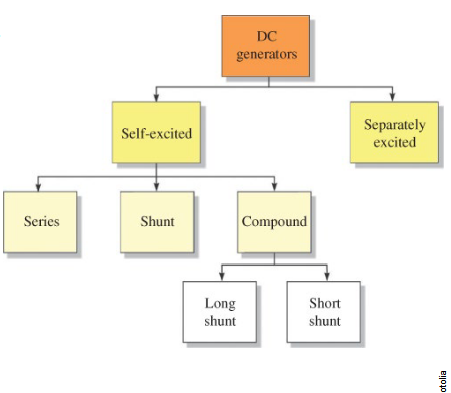
\includegraphics{dc-gen-types.png}
	\end{center}
	Some points to consider are that wil the self-exicted generator, the magnetic field is created through power the generated has made. Compared with a seperately excited generator. Where external power has been supplied.\\
	A note with this is that a shunt generator can be thought of as being in parrellel with itself.\\
	The basics of a generator is shown in the image below. Here the wire loops are wrapped around a shaft (usually iron), which is rotated in the magnet. Power is connected through the brushes only when they are in contact with the communtator. In this example when the wire rotates clockwise, voltage is induced when conductors cut the magnetic flux field. $\therefore$ the maximum power is generated when the conductors are $\perp$ \& a minimum amount when $\sslash$.
	\begin{center}
		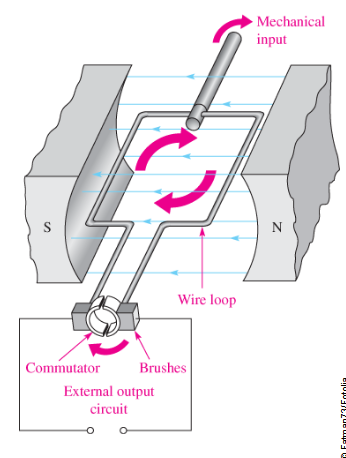
\includegraphics{example-dc-gen.png}
	\end{center}
	To calculate the induced:
	$$V_{ind}=B_{\perp}lv$$
	\begin{itemize}
		\item $V_{ind}$ - Induced Voltage
		\item $B_{\perp}$ - Flux field density ($\frac{\phi}{A}$ in $\frac{Wb}{m^{2}}$ or Telsa(T)
		\item $l$ - length of the wire in the windings (m)
		\item $v$ -Velocity of the motor ($m\;s^{-1}$)
	\end{itemize}
	Graphing this versus its angular position, creates the humps below. To stabilize this into the sterotypical DC voltage, flat line, more wire windings can be used.
	\begin{center}
		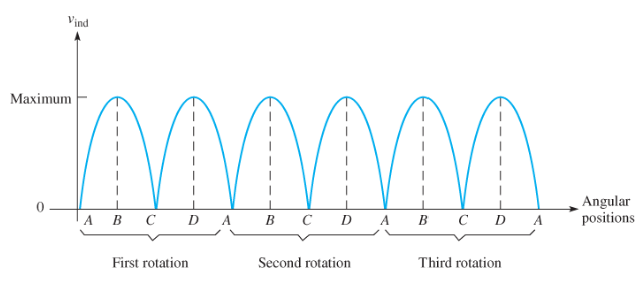
\includegraphics{dc-volt-graph-1}
	\end{center}
	The armature is where the physical voltage is induced. The communtator is where the windings are connected, and copper is used to isolate each winding. If a brush is use, frequent maintainence is required. E.g. to clean the communtator or replace the brush. This is because the brush is made up of carbon.

	\subsection*{Stator Assembly:}
	Field coils (field elctromagnets) generate the magnetic field in the generator. How the coils  recieve current determine their classification. If the generator creates its own current, it is self-exicted. This current is called the excitation current.
	
	\subsection*{DC Generator Types:}
	\subsubsection*{Sperately Excited}
	The current is provided externally. The more amps the wire recieves the greater is magnetic flux. The rheostat is a variable resistor controls the charge current.
	\begin{center}
		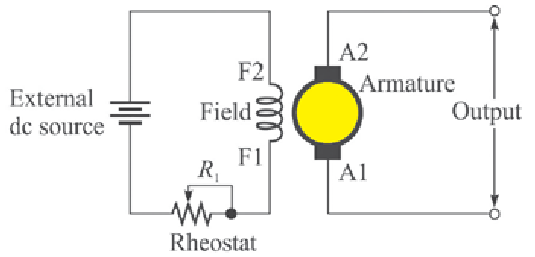
\includegraphics{seperately-excited-dc-gen.png}
	\end{center}
	\subsubsection*{Self-excited}
	The difference between a series and shunt generator is how the armature \& field winding are connected. How it is able to generate enough current to start workings is through a bit of residual magnetisium. Once enough voltage is created to power the windings, power is then generated.
	\begin{center}
		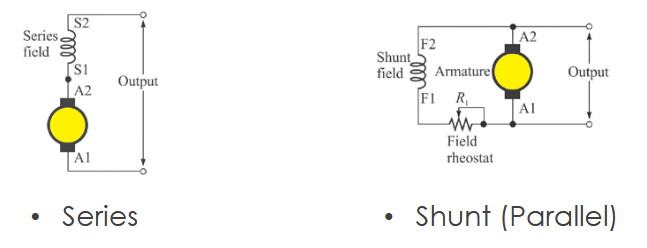
\includegraphics{self-excited-dc-gen.png}
	\end{center}
	\subsubsection*{Compound Generator}
	In compound generators there is two field windings (one series \& one shunt). Depending on where the windings one placed is whether it is a long or short shunt.
	\begin{center}
		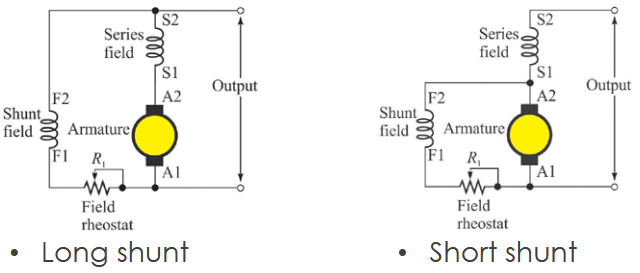
\includegraphics{shunt-dc-gen.png}
	\end{center}

	\subsection*{Polarity of DC Generators:}
	The are two main ways to change voltage in a DC generator:
	\begin{enumerate}
		\item Changing rotation direction of the prime mover. This changes the armatures voltage.
		\item Changing the field winding with respect too the armature winding.
	\end{enumerate}

	\subsection*{AC Synchronous Generators:}
	A synchronous generator is called so because its generated voltage waveform is in sync with the rotation of the generator. There are two main types:
	\begin{enumerate}
		\item Rotating Armature
		\item Rotating Field
	\end{enumerate}
	\subsubsection*{Rotating Field Type}
	Magnetic field is stationary \& supplied by elctromagnets. The output power is taken from the rotor through the brushes and slip rings. All large synchronous generators are rotating field types.
	\begin{center}
		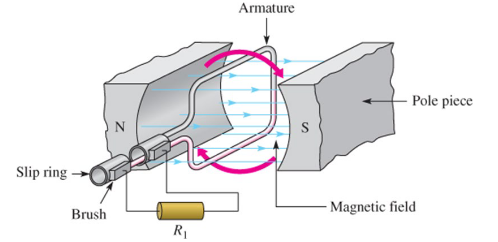
\includegraphics{rotating-field-type-gen.png}
	\end{center}
	\subsubsection*{3-Phase Generator}
	\begin{center}
		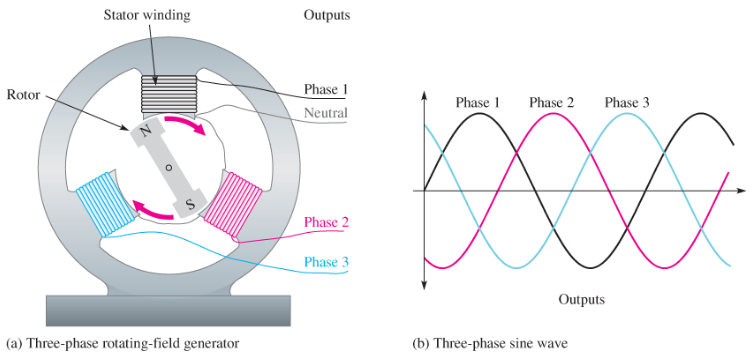
\includegraphics[scale=0.7]{3-phase-ac-gen.png}
	\end{center}
	The frequency of a synchronous generator is determined by the number of poles and speed of rotation.
	$$f=\frac{N_{p}\times RPM}{120}$$
	\begin{itemize}
		\item $f$ - Frequency (Hz)
		\item $N_{p}$ - The number of poles present in the generator
		\item RPM - Revolutions per minute that is does
	\end{itemize}
	\subsubsection*{4-Pole Generator}
	In this generator, 1 revolution produces 2 cycles of the induced voltage waveform.
	
	\subsection*{AC Induction Generators:}
	The AC induction generator is also known as an asynchronous generator. This is because as the waveform in not in sync to the rotational speed.\\
	A bit to understand with this is that this generator can function as either a motor or generator. This is that as the motor's rotor spins at a lesser speed than the synchronous speed, whereas an asynchronous generator's rotor spins faster than the synchronous speed.

	\section*{Weeks 6/7 - Solar Energy:}
	\subsection*{Photovoltaics:}
	These systems are made with silicon semi-conductors.
	\subsubsection*{Semi-conductors}
	Semi-conductors are made out of crystalline silicon (c-Si). Silicon is an element contains a valence band that can possibly have 8 electrons. With this, they will generate a charge with these electrons.
	\subsubsection*{N-Type Silicon}
	When doping silicon with a Group V element. 4 out of 5 valence electrons to form covalent bonds. This makes the semi-conductor slightly negatively charge. Usual doping amount is 100 million Si to 1 Group V element.
	\subsubsection*{P-Type Silicon}
	Here silicon is doped with a Group III element. Creating a slightly positive charge. The missing electron creates what is called a hole.
	\subsubsection*{PN Junctions}
	This junction is formed through a single silicon atom layer, with n-type \& p-type on either side. An example of this is shown in the image below. It is around the depletion region charges can freely move around. This junction is crucial in diodes as the current can only pass in one direction.
	\begin{center}
		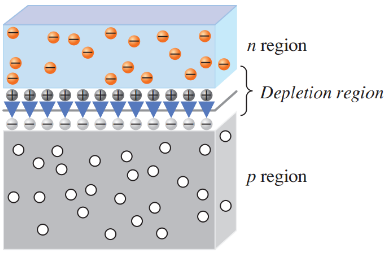
\includegraphics[scale=0.5]{pn-junction.png}
	\end{center}

	\subsection*{PV Cell:}
	An example basic PV cell structure is shown below. When light enters the cell, if the photon energy is greater than the energy gap (1.12eV), a charge will be created.
	\begin{center}
		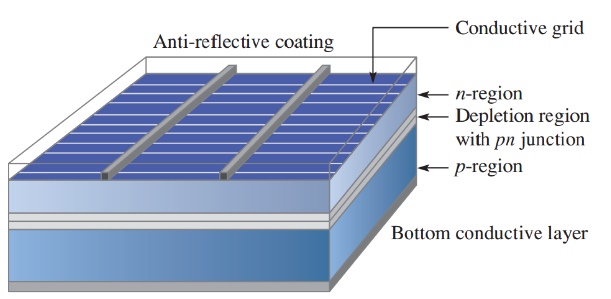
\includegraphics[scale=0.5]{basic-pv-cell.png}
	\end{center}

	\subsection*{Types of PV Cells:}
	There are three main types of PV cells:
	\begin{enumerate}
		\item Monocrystalline - Single cell waffers, providing the highest efficiency
		\item Polycrystalline - Composed of smaller crystals, slightly less efficient
		\item Thin-film - Made of amorphous, the lowest cost to manufacture and least efficient
	\end{enumerate}

	\subsection*{Characteristics of PV Cells:}
	The I-V characteristics is constant a variety of supplied voltages for a specified incident light energy.
	\begin{center}
		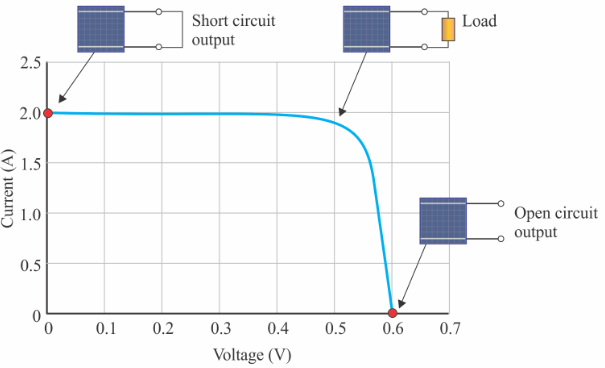
\includegraphics[scale=0.5]{i-v-pv-cells.png}
	\end{center}
	The max power output occurs on the "knee" of the curve.
	\begin{center}
		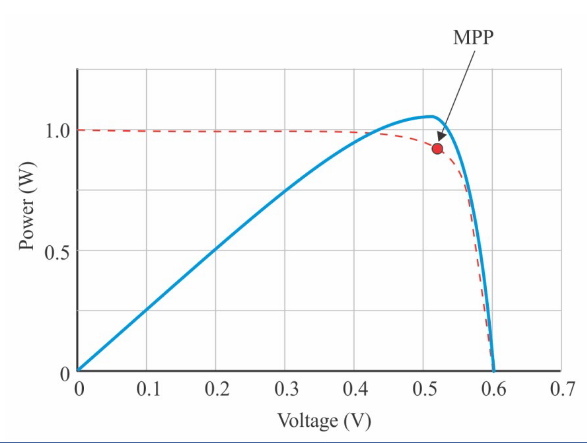
\includegraphics[scale=0.5]{max-pv-power.png}
	\end{center}
	On the back of each module is a junction box, containnig two standardized cables. These connect the modules. When connecting modules in series it is called a string. Multiple different strings can be connected in parrallel to form an array.The whole system is a combiner.

	\subsection*{Solar Power System:}
	Stand-alone systems do not power the grid. Rather are used for smaller, remote applications. Most systems are only DC @ 12, 24, 48V. When using a solar cell to charge a battery, a charge controller is used to regulate \& limit the charging rate. So as to not over charge the battery.

	\subsection*{Sizing the System:}
	$$P_{array}=\frac{W}{t_{solar}\;\eta_{sys}}$$
	\begin{itemize}
		\item $P_{array}$ - W
		\item $W$ - Wh
		\item $t_{solar}$ - Number of hours of solar a day
		\item $\eta_{sys}$ - Efficiency of the system
	\end{itemize}
	$$Ah=\frac{W_{day}\;t_{store}}{V\;B_{DoD}\;\eta_{inv}}$$
	\begin{itemize}
		\item Ah - Amphours for the battery
		\item $W_{day}$ - $\frac{Wh}{day}$
		\item $t_{store}$ - The number of days the battery needs to provide power (days)
		\item $V$ - Dc system voltage to the inverter
		\item $B_{DoD}$ - Batteries max depth of discharge
		\item $\eta_{inv}$ - Efficiency of the inverter
	\end{itemize}
	$$FF=\frac{P_{MPP}}{V_{OC}\;I_{SC}}$$
	This describes how close the PV cell is to the theoretical maximum efficiency.

	\subsection*{Solar Concentrators:}
	A SC uses either mirrors or lenses to focus the light upon a point. A mirror system assumes the light comes in parrallel to the mirror. This is then reflected to a point on the axis called the focal point($f_{p}$). The $f_{p}$ is always $\frac{1}{2}r_{c}$.
	\begin{center}
		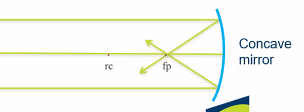
\includegraphics{concave-mirror.png}
	\end{center}
	When the light passes through a lense, a convex one is used. Because of costs, lense systems are not widely used.
	\begin{center}
		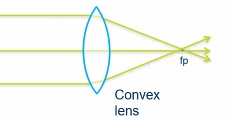
\includegraphics{convex-lens.png}
	\end{center}

	\subsection*{Concentrated Solar Power:}
	CSP system can be used to store thermal energy in a fluid, then use it whenever it is needed. It works similar to the traditional steam engine.
	
	\subsection*{Solar Hot Water Systems:}
	Solar hot water systems work through fluid-plate collectors, focusing sunlight on a manifold to heat the water. The manifold's pipes are usually coverede in a material that has a high absorbance. In areas subject to freezing a closed-loop, pressurized glycol-water system will have to be used.

	\subsection*{Solar Movement:}
	Remember the earth GPS with latitudes and longitudes. The earth is on a $23.4^{o}$ include to equator. It is important to know this to understand the amount of sunlight on the earth.
	\subsubsection*{Solar Tracking}
	Solar cells work best with direct sunlight. Trackers follow the Sun's direction throughout the day. Increasing the time that the cells can achieve maximum efficiency. Single axis tracking only does East-West movement. Whereas dual axis can also move North-South. Within these there are two types of trackers.
	\begin{enumerate}
		\item Active - Using actual motors
		\item Passive - Uses liquid \& gas properties to move the cell
	\end{enumerate}

	\subsection*{Other Equations to Know:}
	$$\tau =K\phi I_{a}$$
	$$\tau = \frac{P}{\omega}$$
	\begin{itemize}
		\item $\tau$ - Torque ($N\cdot m$)
		\item K - $N\cdot m\;\text{or}\;Wb\cdot A$
		\item $\phi$ - Wb
		\item $I_{a}$ - A in the armature
		\item $P$ - Power (W)
		\item $\omega$ - $\frac{rad}{s}$
	\end{itemize}
	$$V_{S}=C_{emf}+I_{a}R_{a}$$
	\begin{itemize}
		\item $V_{S}$ - The applied voltage
		\item $C_{emf}$ - Counter EMF (V)
		\item $I_{a}R_{a}$ - Their respective items in the armature
	\end{itemize}

	\section*{Week 8 - Wind Energy:}
	\subsection*{Air Pressure:}
	The pressure of the air (air pressure) is crucial to the wind systems.
	$$P=\frac{F}{A}$$
	\begin{itemize}
		\item $P$ - Pressure (Pa)
		\item $F$ - Force (N)
		\item $A$ - Area ($m^{2}$)
	\end{itemize}
	$$1mbar\;=\;100Pa$$
	$$1atm\;=\;101320Pa$$
	$$1mmHg\;=\;133.3Pa$$
	$$1psi\;=\;6895Pa$$
	A sea breeze is formed in a temperature difference between the water \& the land. The laminar flow is when a liquid (or gas) moves in a straight line. The opposite of this is turbulent flow. The change in velocity behind the turbine creates a turbulent zone, the zone is expandend by this air mixing with the normal air speed.

	\subsection*{Wind Turbine:}
	\begin{center}
		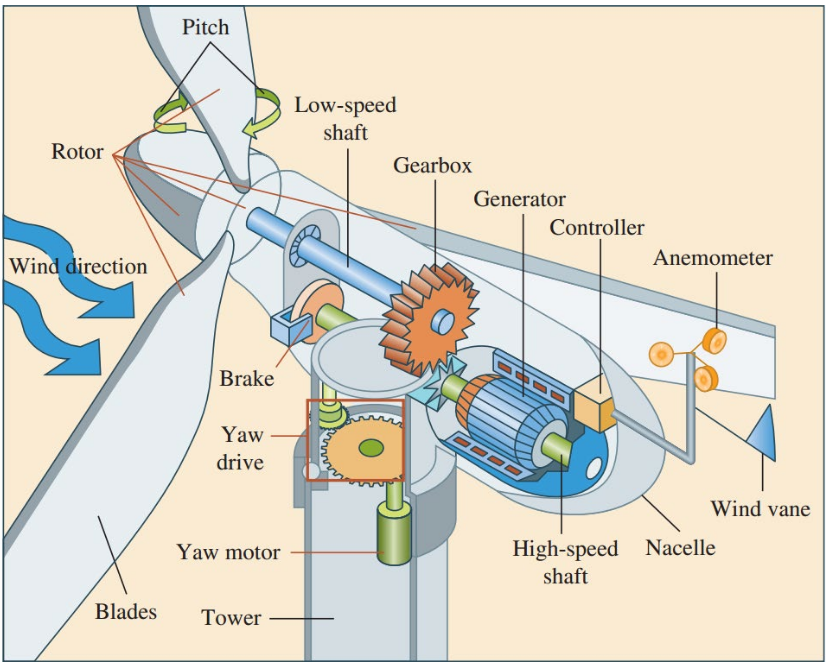
\includegraphics[scale=0.5]{basic-turbine-diagram.png}
	\end{center}
	$$P_{w}=\frac{1}{2}A\rho_{a}v_{w}^{3}$$
	\begin{itemize}
		\item $P_{w}$ - Power Generated by the turbine (W)
		\item $A$ - Area cut by the turbine blades ($m^{2}$)
		\item $\rho_{a}$ - Density of air ($\frac{kg}{m^{3}}$)
		\item $v_{w}$ - Velocity of the wind ($\frac{m}{s}$)
	\end{itemize}

	\subsection*{Betz's Law:}
	Betz's Law describes the theoretical maximum efficiency of a turbine (59.3\%). However, the real efficiency will be much lower in real-world applications, through friction.

	\subsection*{Horizontal Axis Wind Turbine:}
	A HAWT is the most common type of turbine. For it to bo connected straight to the grid the frequency of AC output must match the grid's. In Australia this is 50Hz. To do this different methods are used:
	\begin{enumerate}
		\item Generator Shaft Speed.\\
		$$n_{s}=\frac{120f}{N_{p}}$$
		\begin{itemize}
			\item $n_{s}$ - RPM
			\item $f$ - Frequency (Hz)
			\item $N_{p}$ - No. of Poles
		\end{itemize}
		\item Frequency Converter:\\
			AC->DC->AC->Act Transformer
		\item Double-fed
		\begin{center}
			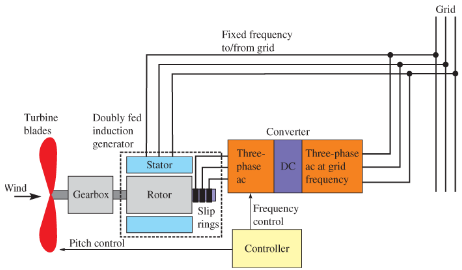
\includegraphics[scale=0.5]{double-fed-turbine.png}
		\end{center}
	\end{enumerate}

	\subsection*{Wind Farms:}
	The turbines offer the adventage of scale. Containing the ability to share maintainance.\\
	Offshore wind farms are gaining popularity. This is due to no obstacles in the way (e.g. mountains or houses) and uniform windspeeds (e.g. again nothing in the way).

	\subsection*{Pitch \& Yaw:}
	Pitch control allows controlling the angle the blade to control the turbine speed. Usually controlled by hydraulic actuaters in a 4-20mA loop. Yaw control points the direction of the turbine. It orients the "centre" of wind by the blades before the nacelle.

	\subsection*{Drive-train:}
	Most turbines rotate @ 20rpm. The gearbox increases this to 1500-1800rpm. 

	\section*{Week 9 - Hydro Power:}
	\subsection*{Types of Hydro:}
	\subsubsection*{Dam}
	Water from the dam flows through penstocks. They direct it ot the turbine to the generate power and electricity.
	\subsubsection*{River}
	Uses the $K_{E}$ of the running water to generate the electricity.

	\subsection*{Types of Turbines:}
	The first type is the impulse turbine. It is primarily used in applications with high pressure \& low flow rates. The second type is the reaction turbine. These are usually submerged in water and develop a torque from differential water pressures. The third type is cross flow turbines. These have the water flow across the turbine.

	\subsection*{Tidal:}
	$$W_{PE}=\frac{1}{2}\rho Agh^{2}$$
	\begin{itemize}
		\item $W_{PE}$ - Water's potential energy (J)
		\item $\rho$ - Density of water ($\frac{kg}{m^{3}}$)
		\begin{itemize}
			\item Saltwater - $1220\frac{kg}{m^{3}}$
			\item Fresh water - $1000\frac{kg}{m^{3}}$
		\end{itemize}
		\item $A$ - Area ($m^{2}$)
		\item $g$ - Gravity ($9.8\frac{m}{s^{2}}$)
		\item $h$ - $\frac{1}{2}h_{max}$
	\end{itemize}

	\subsection*{Conversion Fractors:}
	\begin{center}
		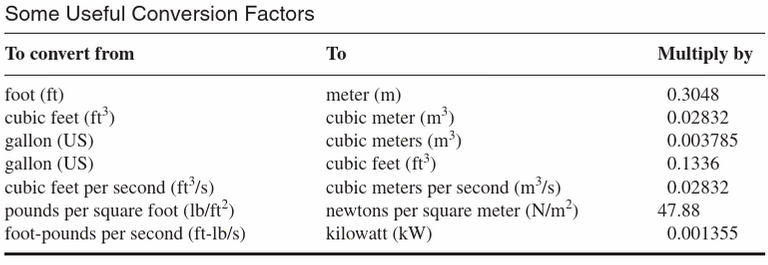
\includegraphics[scale=0.5]{si-conversion-fractors.png}
	\end{center}

	\section*{Week 10 - Hydrogen, Fuel Cells and Enenrgy Storage:}
	\subsection*{Hydrogen:}
	Hydrogen is the most common element in the world (~75\% of the mass). Focusing upon earth, hydrogen can be found everywhere and nearly all living things. However, hydrogen is very rarely in pure gaseous form (1ppm). As such hydrogen must be extracted from larger molecules.
	\hfill\break\break
	The oxidation (burning) of hydrogen generates thermal energy. Unlike other form of fossil fuel combustion (complete $CO_{2}$ or incomplete $CO$), hydrogen only form water. Since burning hydrogen does not produce visible light it is much more efficient. Hydrogen generates 120-142$\frac{MJ}{kg}$. However, to store hydrogen is must be cooled to almost 0K.
	
	\subsection*{Hydrogen Colour Spectrum:}
	Hydrogen is colour-less gas, however there is a colour-coded table (below) to identify the method of production.
	\begin{center}
		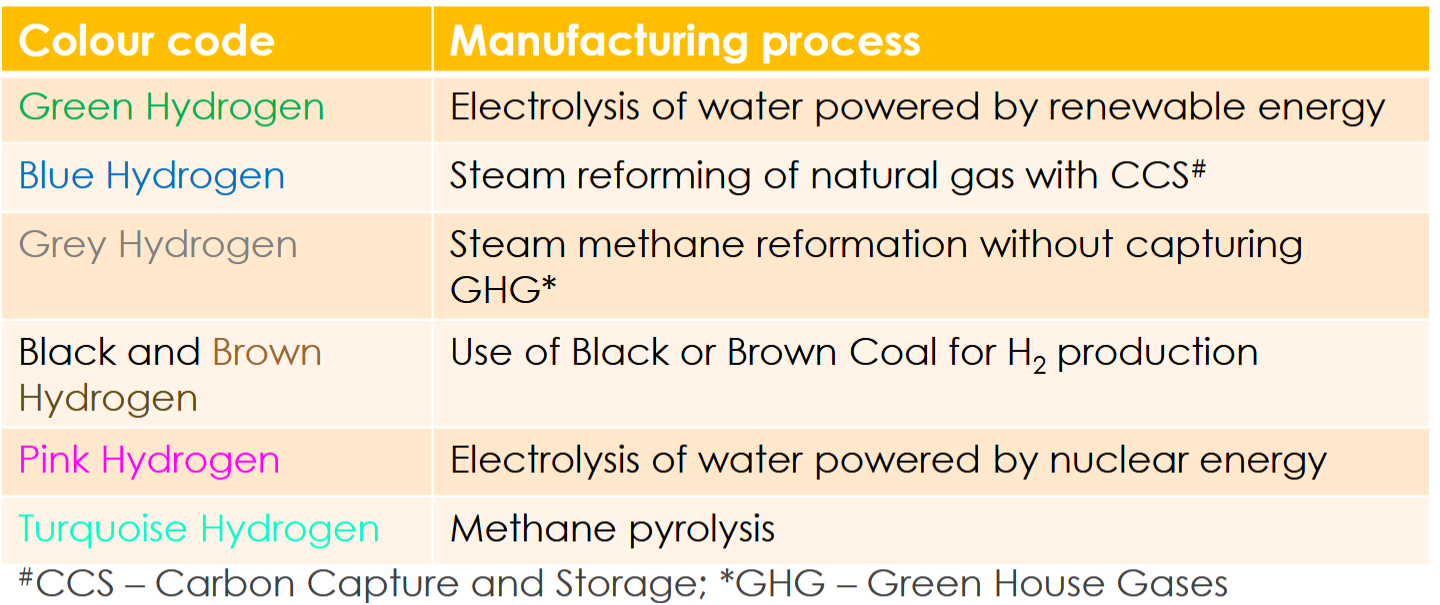
\includegraphics[scale=0.5]{h-table.png}
	\end{center}
	\subsubsection*{Electrolysis of Water}
	This utilizes an electrical current through water to create pure hydrogen and oxygen.
	\subsubsection*{Blue Hydrogen}
	Created through the steam reformation of a natural gas (usually methane) in the presence of the a catalyst.
	$$CH_{4(g)}+H_{2}O_{(g)}<->CO_{(g)}+3H_{2(g)}$$
	$$CO_{(g)}+H_{2}O_{(g)}<->CO_{2(g)}+H_{2(g)}$$

	\subsection*{Fuel Cells:}
	A fuel cell is a device that converts electrochemical energy from a substance into a direct current. This is similar to a battery, bu the fuel can be stored outside of the reaction area. The chemical reaction (oxidation) occurs releasing the electron and producing electricity. Just remember the HFC and LEFC from chemistry research.
	\subsubsection*{REDOX Reactions}
	A reactant loses electrons (oxidation) and the other gains the electrons (reduction). These electrons travel through a wire generating a current. For the charges in the cell, remember anodes are negative and cathodes are positive.
	\newpage
	\begin{itemize}
		\item Oxidation
		\item Is
		\item Loss
		\item Reduction
		\item Is
		\item Gain
	\end{itemize}
	There are three main fuel cell system:
	\begin{enumerate}
		\item Fuel Cell Stack: A group of fuel cell connected together to increase the outputted power.
		\item Fuel Processing Unit: The process the converts the fuel into usable form for the reaction.
		\item Heat Exchange Unit: Captures some excess heat generated during the reaction.
	\end{enumerate}
	\subsubsection*{Types of the Fuel Cells}
	The fuel cells describe the chemistry and physical makeup of the cell.
	\begin{center}
		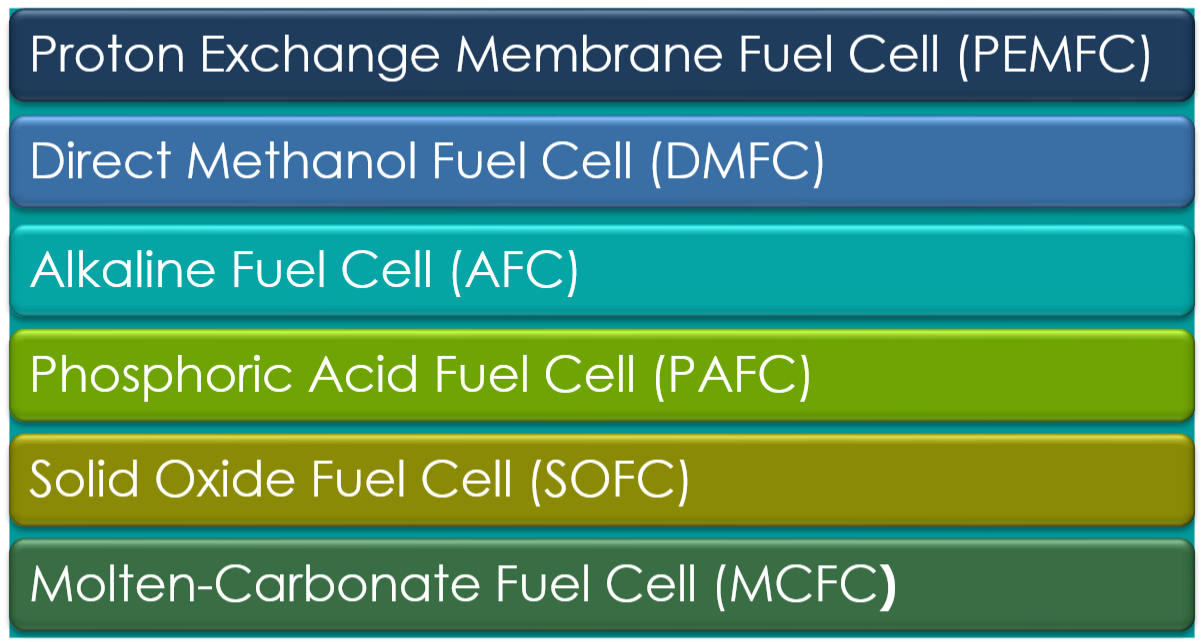
\includegraphics[scale=0.5]{fuel-cell-type.png}
	\end{center}

	\subsection*{Primary \& Secondary Energy:}
	Primary energy is the naturally found energy souces. These include oil, coal, waste, biomass, or wind. Once these undergo a transformation into a usable form, they become secondary energy sources. Petroleum products, electricity or biofules.
	
	\subsection*{Energy Storage:}
	The storage of excess energy is an essential link in the energy supply chain. The most basic form is batteries for renewable energy. This is because they supply intermittent outupts, creating an unrealiable form of energy supply. Energy storage stores the excess energy when it is generated and suppliment when extra power is required. 
	\subsubsection*{Mechanical - Flywheel}
	The flywheel is stored in a low friction environment. It smoothes out power and continues generation through the $K_{E}$ being stored in its rotation. To connect it to the grid, and electrical machine used intially as a motor to convert electricity into movement and then power is needed, it is used as a generator.
	\subsubsection*{Mechanical - Pumped Hydro}
	Just remeber the hydro from Week 9. Here there are two main types. 
	\begin{enumerate}
		\item Open-loop: Lower reservior is part of a running river. The upper reservior is an extra lake.
		\item Closed-loop: The upper and lower reservior are two seperate system, not part of running water.
	\end{enumerate}
	\subsubsection*{Electrochemical - Batteries}
	\begin{center}
		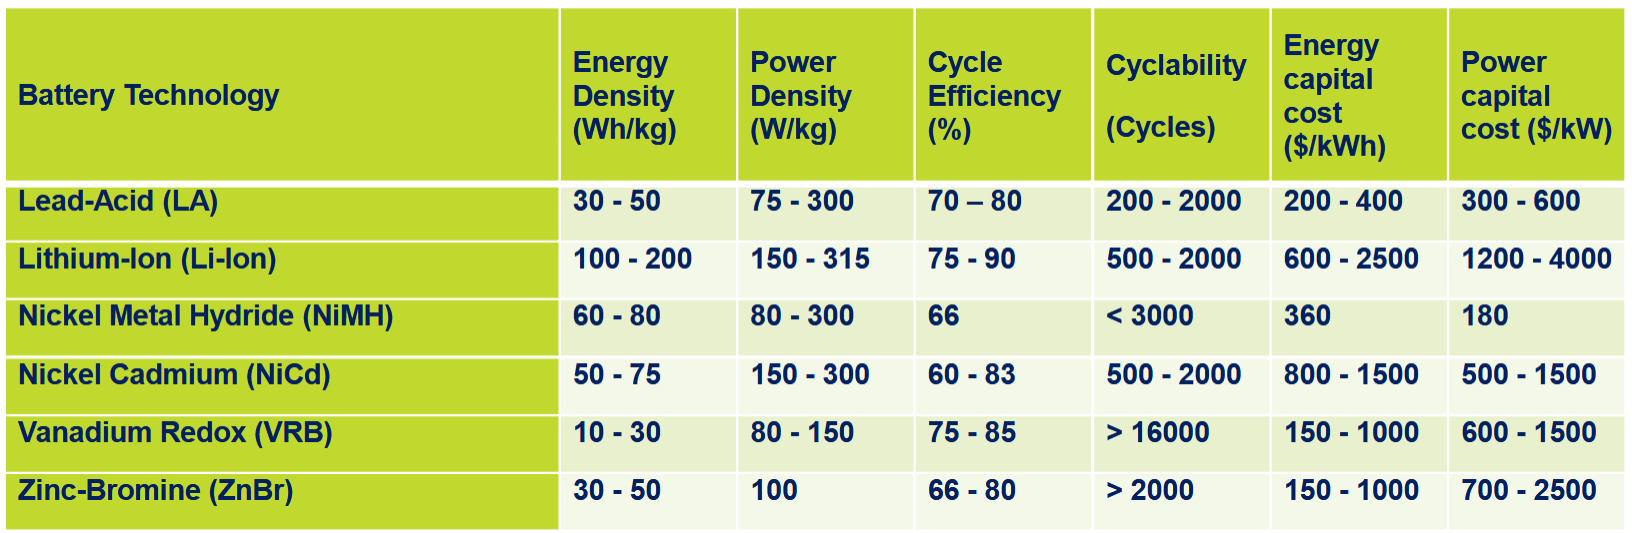
\includegraphics[scale=0.4]{battery-type.png}
	\end{center}
\end{document}
